% ansys, 12543*2 2nd order 4.92747
% ansys(1st)
% 100*2 - 4.82274
% 361*2 - 4.89143 
% 1369*2 -4.91566
% 5328*2 -4.92411
% err_a1 = abs([4.82274,4.89143,4.91566,4.92411]-4.92747)/4.92747; dof_a1 = [100,361,1369,5328]*2; polyfit(log(dof_a1), log(err_a1),1)


% ansys(2nd)
% 133*2 - 4.88648
% 481*2 - 4.91409
% 1825*2 - 4.92356
% 7105*2 -  4.92685
% err_a2 = abs([4.88648,4.91409,4.92356,4.92685]-4.92747)/4.92747; dof_a2 = [133,481,1825,7105]*2; polyfit(log(dof_a2),log(err_a2),1)

% svm
% 162 - 4.82
% 426 - 4.8945
% 992 - 4.9131
% 1780 - 4.9175
% 2614 - 4.9208
% err = abs([4.82,4.8945,4.9131,4.9175,4.9208] - 4.92747)/4.92747; dof=[162,426,992,1780,2614]; polyfit(log(dof),log(err),1)

% mlp
% 162-4.82
% 496-4.8884
% 1014-4.9090
% 1202-4.9151
% 3146-4.9226
% err = abs([4.82,4.8842,4.9060,4.9180,4.9226] - 4.92747)/4.92747; dof=[162,420,808,1484,3146]; polyfit(log(dof),log(err),1)

\subsection{Short cantilever beam}
\paragraph{}
A two-dimensional short cantilever beam subjected to a uniformly distributed load at the top is examined as shown
in Fig.~\ref{adp_fig:ex_cantilever_beam_geo_bc}.
    \begin{figure}[h!]
    \centering
        \scalebox{0.5}{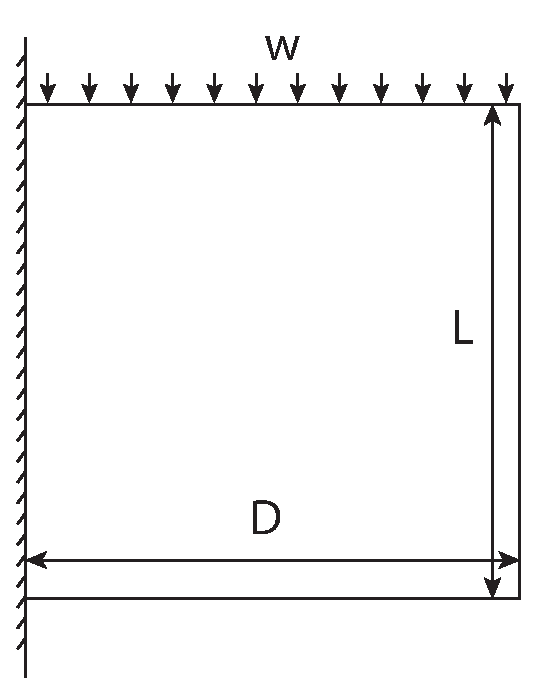
\includegraphics{adaptivity/ex_images/ex_short_cant_geo_bc.eps}}
        \caption{ Short cantilever beam: Geometry and boundary conditions.}
        \label{adp_fig:ex_cantilever_beam_geo_bc}
    \end{figure}

The geometry is: length $L = \SI{1}{\meter} $, height $ D = \SI{1}{\meter} $.
The material properties are: Young’s modulus $ E = \SI{20}{\newton \per \meter^2} $ , Poisson’s ratio $ \nu =0.3 $.
The uniformly distributed load is $w = \SI{10}{\newton \per \meter} $.
Plane stress is assumed.

The reference strain energy of \SI{4.02079}{\joule} is determined by the help of ANSYS.
In ANSYS, a mesh with $17930$ DOF using 2 \textsuperscript{nd} order plane element 183 is used to calculate the result.

Due to the fact that the geometry of the cantilever beam can be described by four points and four straight lines, drawing in AutoCAD may not be necessary.
As a result, the input geometry is defined manually.


\paragraph{}
The numerical convergence of the the relative error in the energy norm is shown in Fig.~\ref{adap_fig:ex_short_cantilever_convergence}.
It can be observed that data mining based adaptive SBFEM yield superior convergence rate when compared to result calculated in ANSYS.

\begin{figure}[h!]
    \centering
    \scalebox{0.5}{
        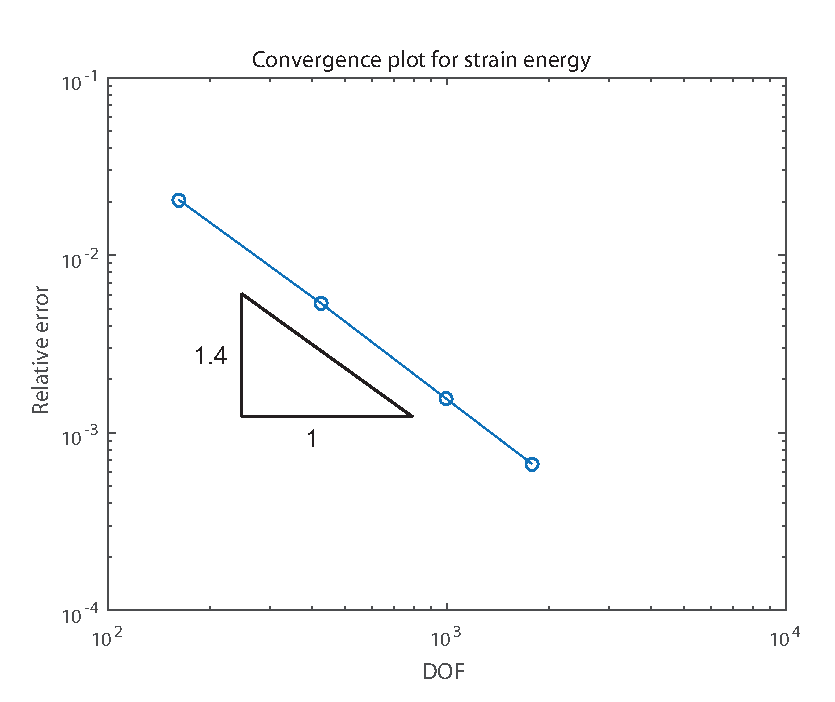
\includegraphics{adaptivity/ex_images/ex_short_cantilever_conv.eps}
    }
    \caption{the relative error in the energy norm}
    \label{adap_fig:ex_short_cantilever_convergence}
\end{figure}

Corresponding mesh development are plotted in Fig.~\ref{adap_fig:ex_short_cantilever_mesh_develpment} (SBFEM 1\textup{st} order element) and Fig.~\ref{adap_fig:ex_short_cantilever_mesh_develpment_ansys} (ANSYS 9-node quadrilateral element).
Stress contour plot in ANSYS using 9-node quadrilateral elements (17930 DOFs) are shown in Fig.~\ref{adap_fig:ex_chole_stress_ansys}
\begin{figure}[h!]
\centering
    \begin{subfigure}[b]{0.4\linewidth}
        \centering
        \scalebox{0.25}{
            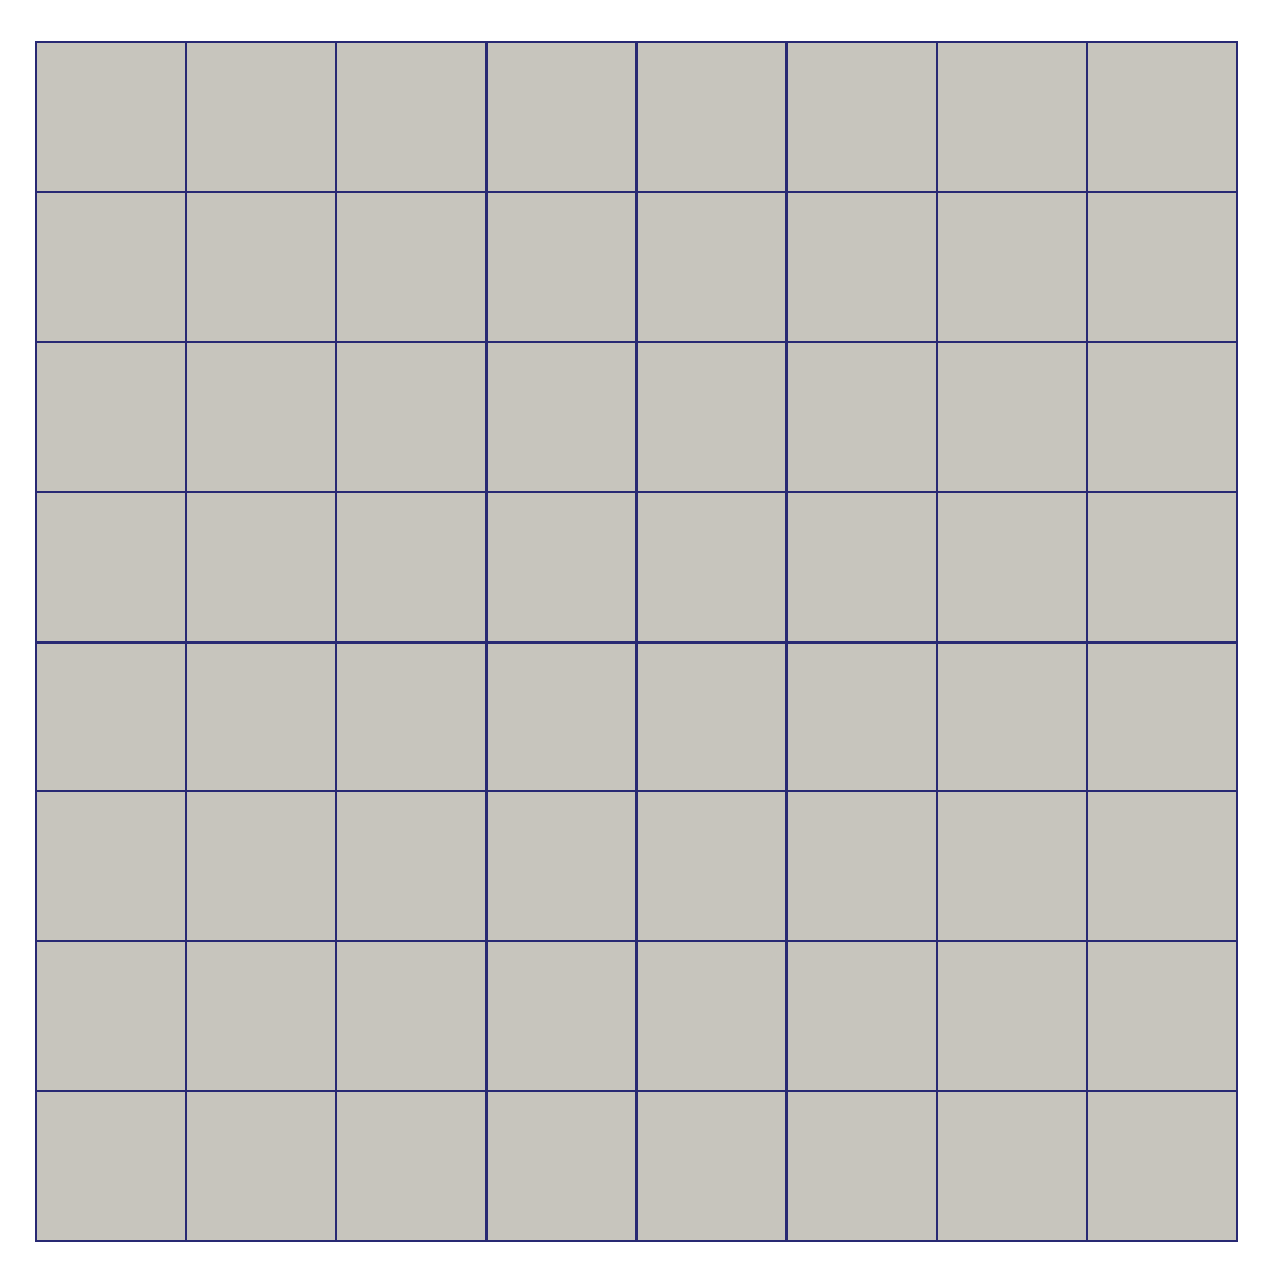
\includegraphics{adaptivity/ex_images/ex_short_cantilever_mesh_162.eps}
        }
        \caption{Initial mesh (162 DOF)}
    \end{subfigure}
    \begin{subfigure}[b]{0.4\linewidth}
        \centering
        \scalebox{0.25}{
            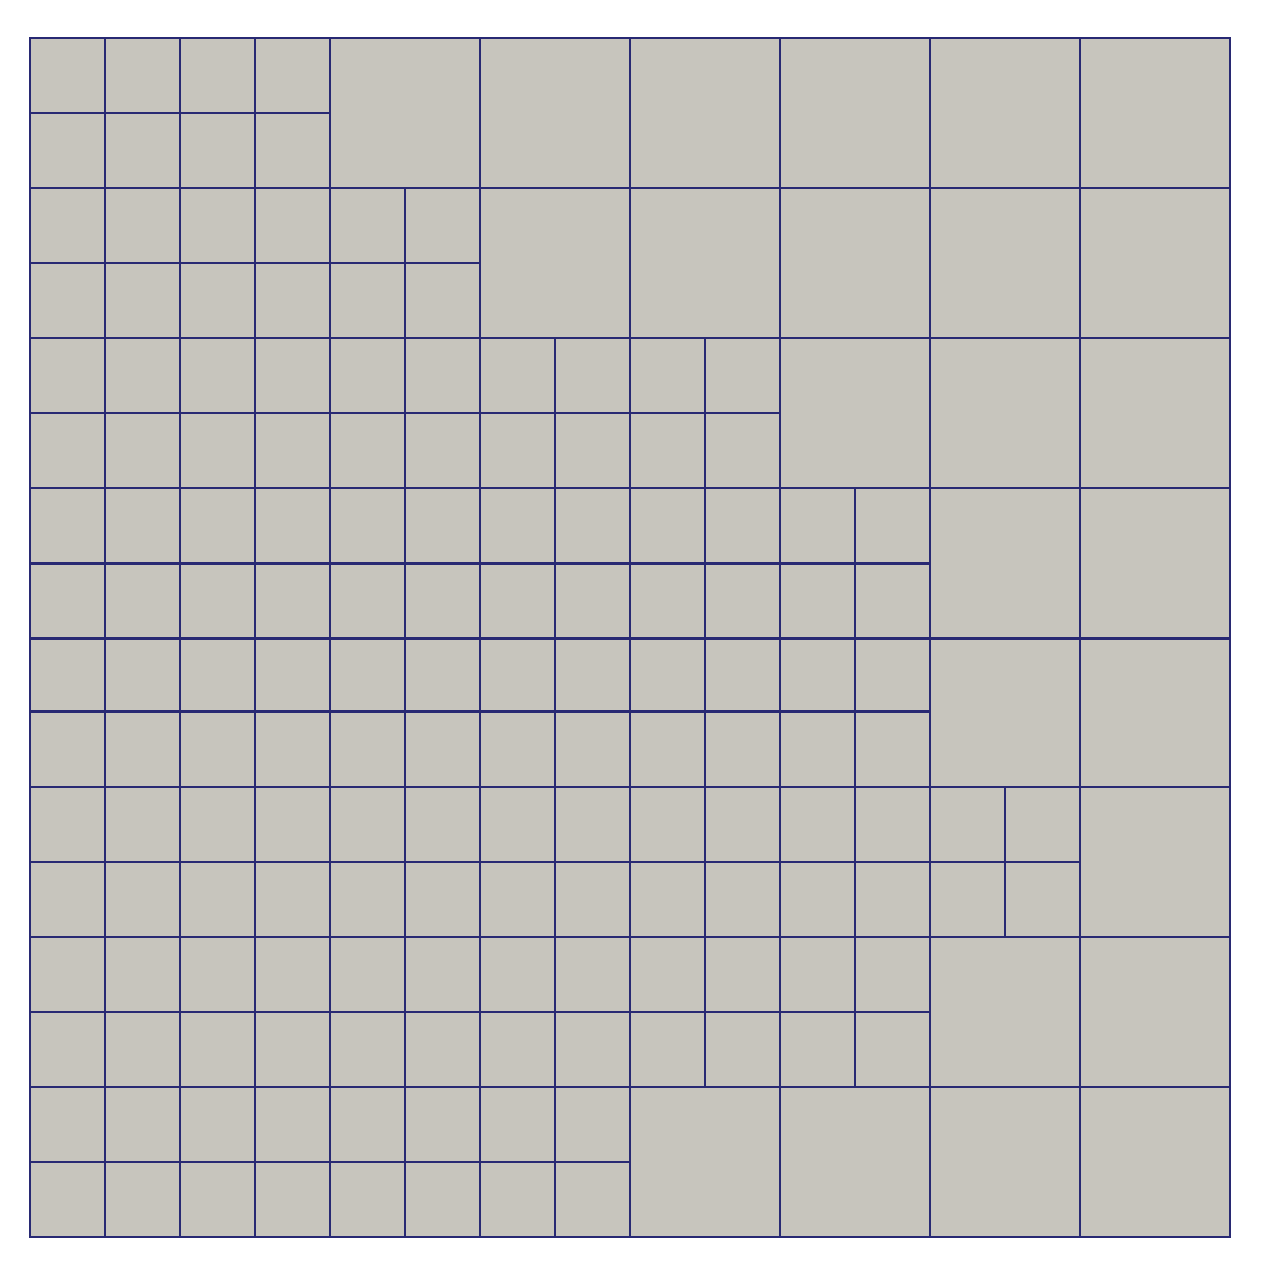
\includegraphics{adaptivity/ex_images/ex_short_cantilever_mesh_462.eps}
        }
        \caption{1st refinement (462 DOF)}
    \end{subfigure}
    \begin{subfigure}[b]{0.4\linewidth}
        \centering
        \scalebox{0.25}{
            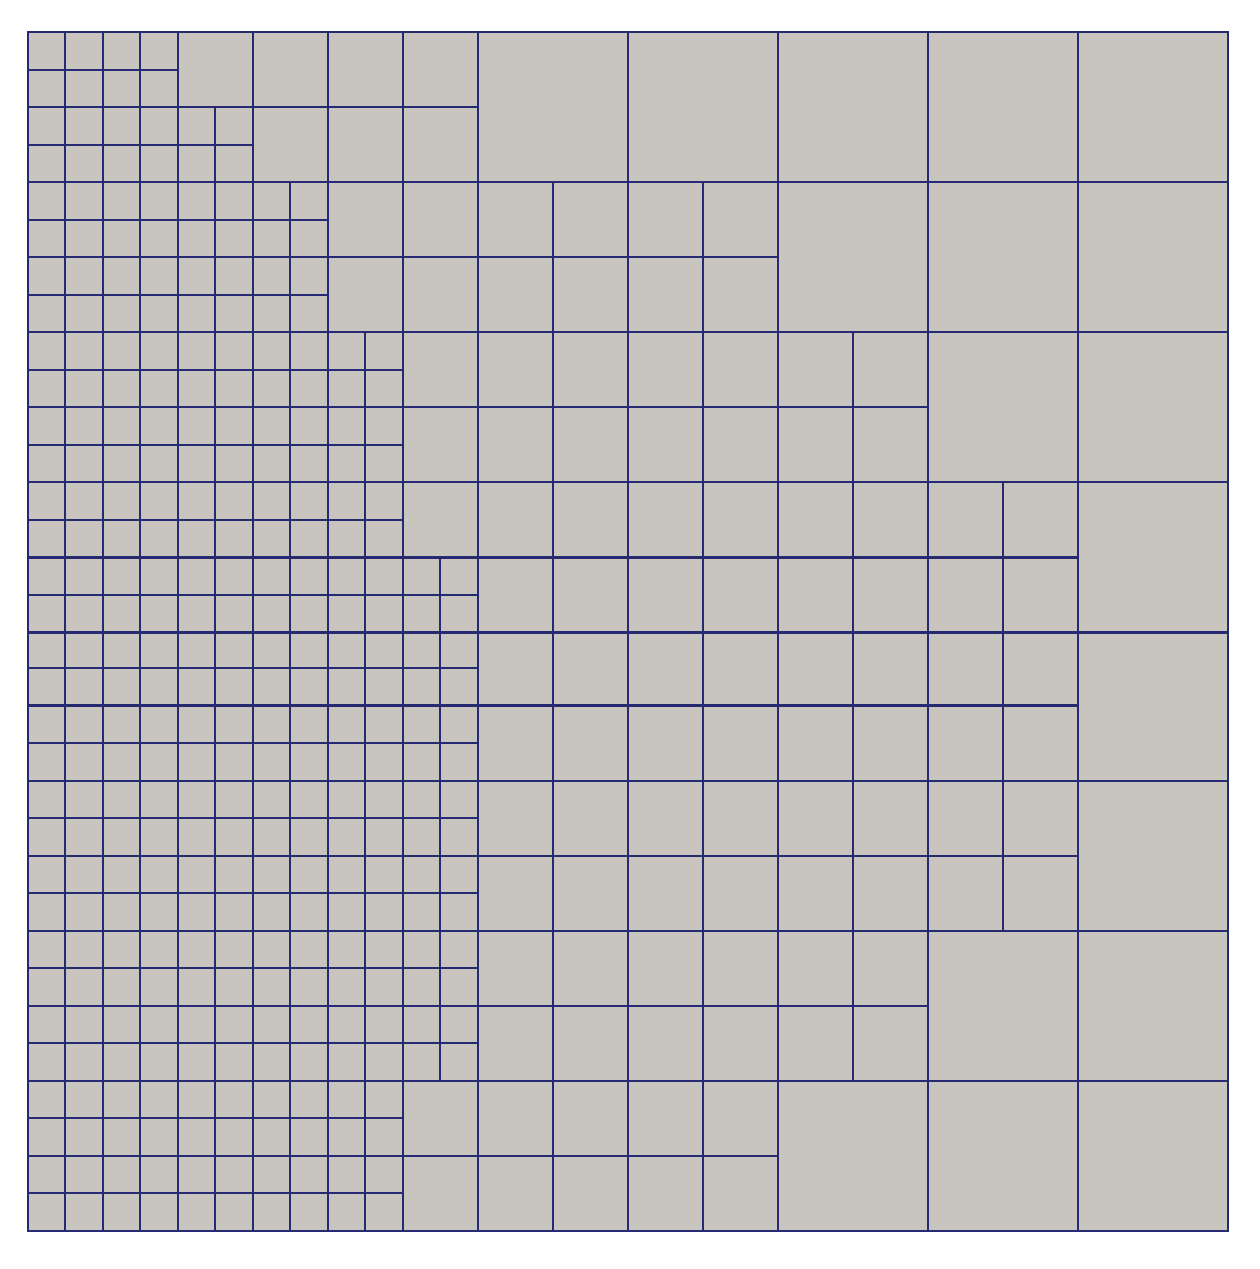
\includegraphics{adaptivity/ex_images/ex_short_cantilever_mesh_992.eps}
        }
        \caption{2nd mesh (992 DOF)}
    \end{subfigure}
    \begin{subfigure}[b]{0.4\linewidth}
        \centering
        \scalebox{0.25}{
            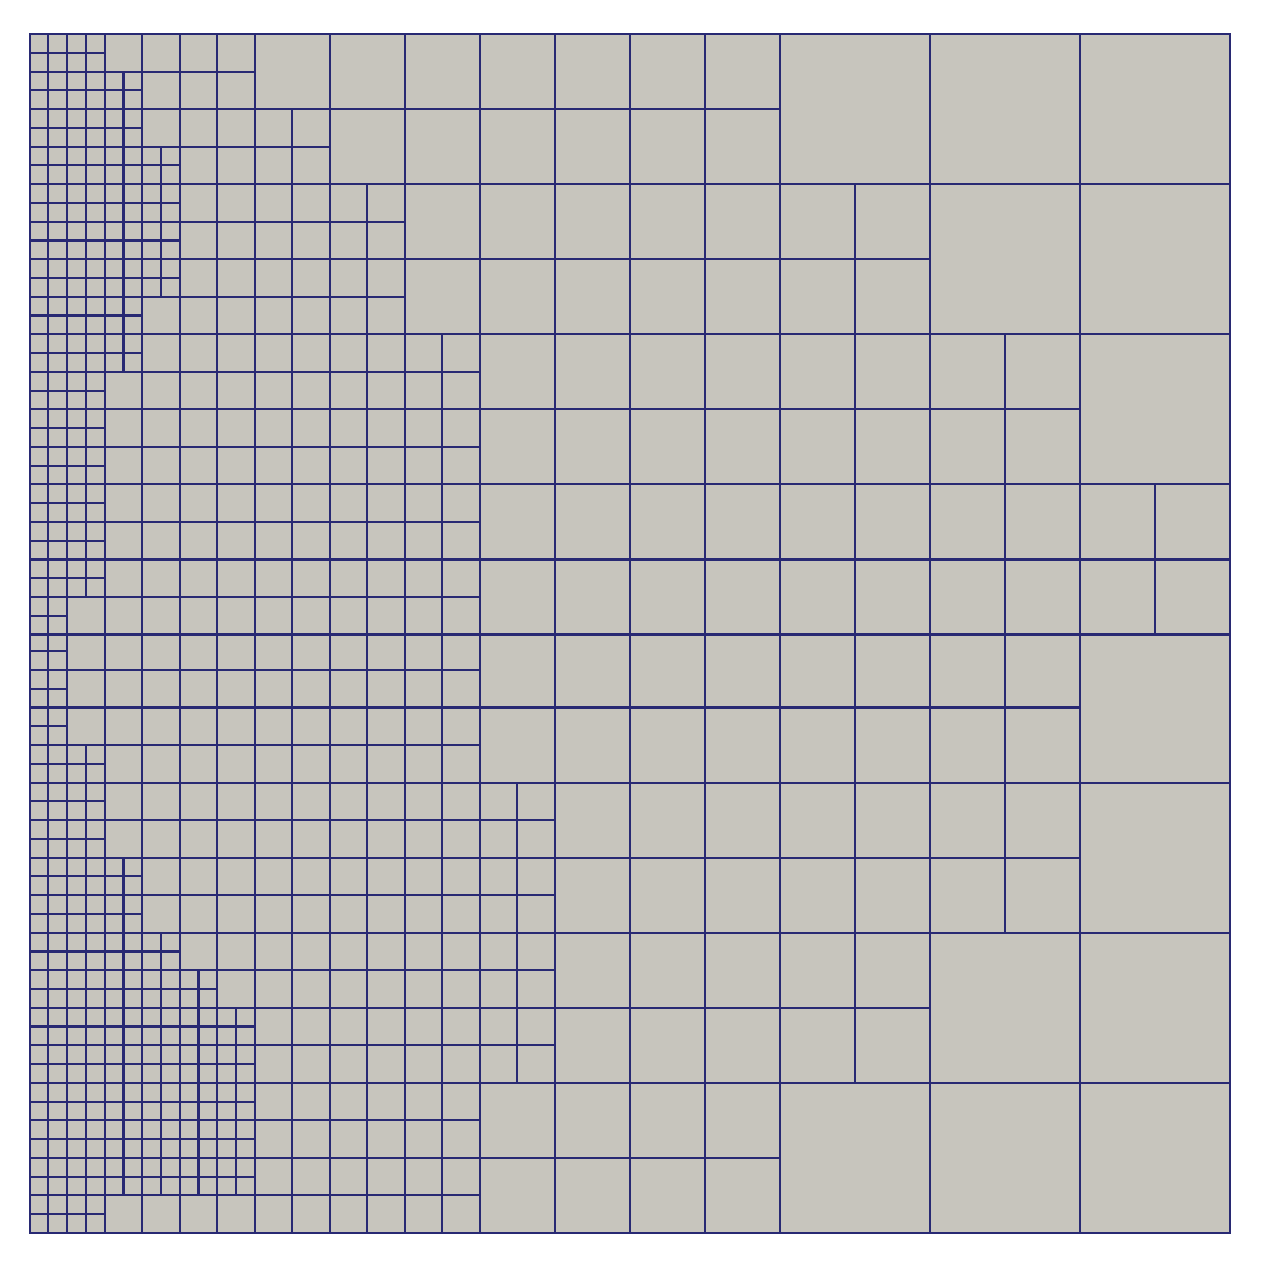
\includegraphics{adaptivity/ex_images/ex_short_cantilever_mesh_1780.eps}
        }
        \caption{3rd refinement (1780 DOF)}
    \end{subfigure}
    \caption{ Short cantilever beam: mesh development (SBFEM)}
    \label{adap_fig:ex_short_cantilever_mesh_develpment}
\end{figure}

\begin{figure}[h!]
    \centering
    \begin{subfigure}[b]{0.48\linewidth}
        \centering
        \scalebox{0.35}{
            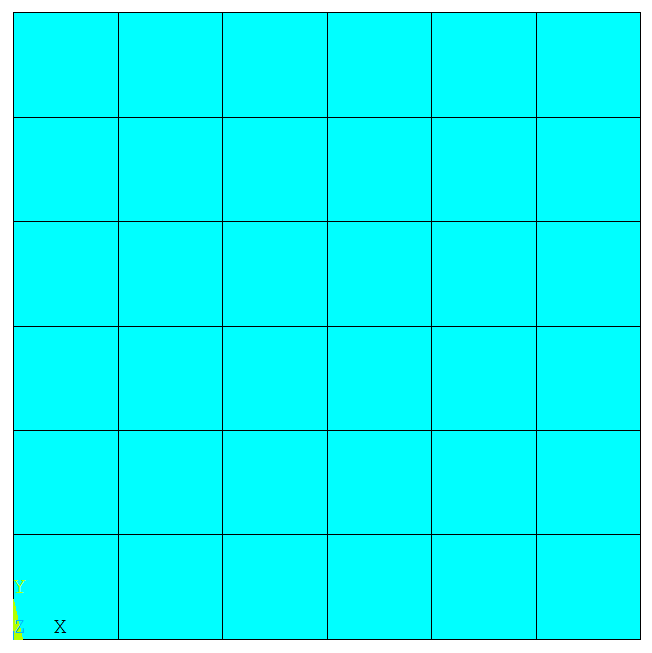
\includegraphics{adaptivity/ex_images/ex_short_cantilever_ansys_2_133.png}
        }
        \caption{Initial mesh, 266 DOFs}
    \end{subfigure}
    \begin{subfigure}[b]{0.48\linewidth}
        \centering
        \scalebox{0.35}{
            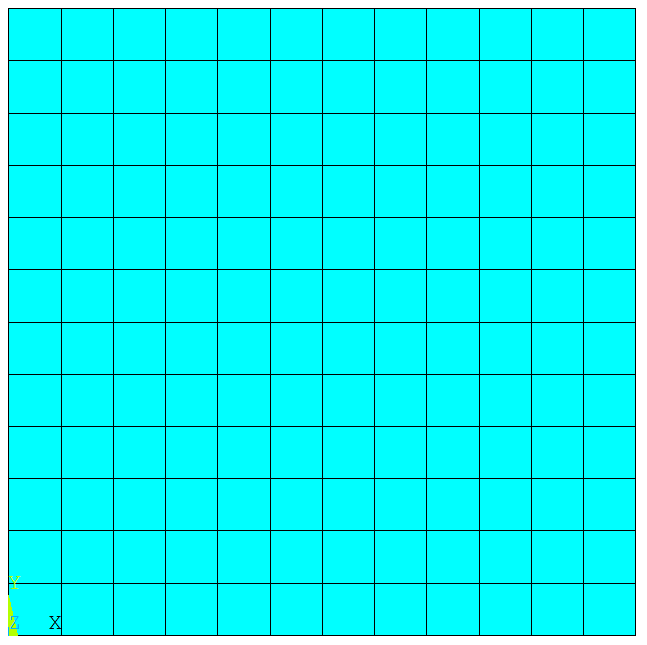
\includegraphics{adaptivity/ex_images/ex_short_cantilever_ansys_2_481.png}
        }
        \caption{1st refinement, 962 DOFs}
    \end{subfigure}
    \begin{subfigure}[b]{0.48\linewidth}
        \centering
        \scalebox{0.35}{
            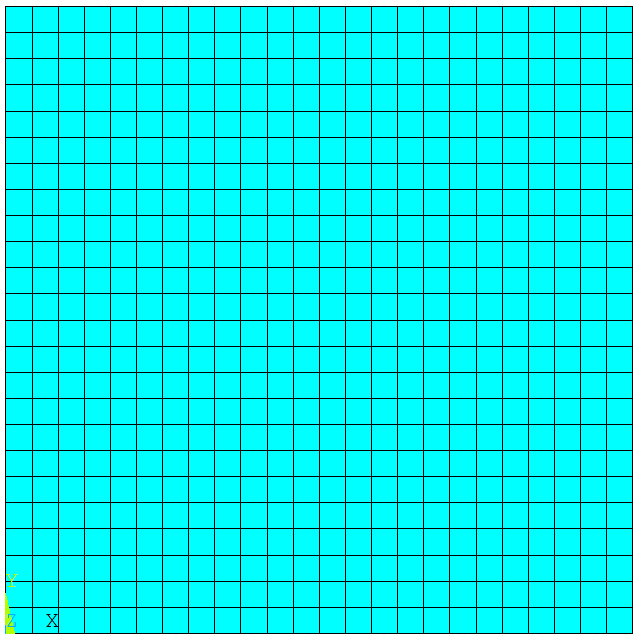
\includegraphics{adaptivity/ex_images/ex_short_cantilever_ansys_2_1825.png}
        }
        \caption{2nd refinement, 3650 DOFs}
    \end{subfigure}
    \begin{subfigure}[b]{0.48\linewidth}
        \centering
        \scalebox{0.35}{
            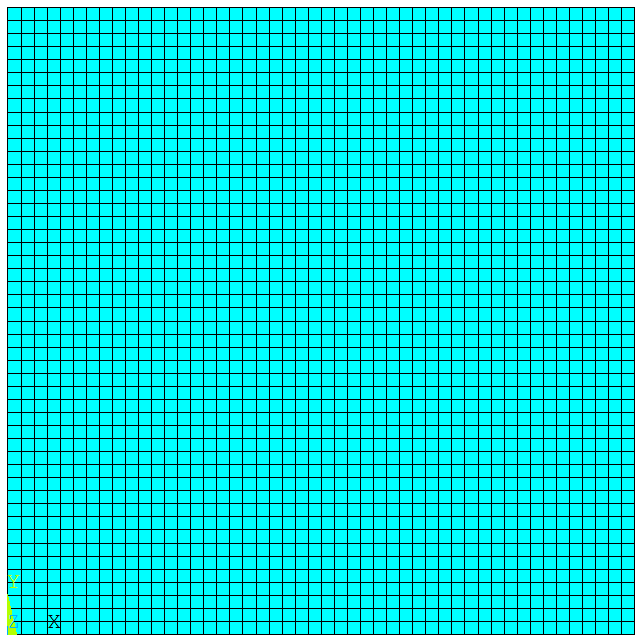
\includegraphics{adaptivity/ex_images/ex_short_cantilever_ansys_2_7105.png}
        }
        \caption{3rd refinement, 14210 DOFs}
    \end{subfigure}
    \caption{Short cantilever beam: mesh development (Ansys)}
    \label{adap_fig:ex_short_cantilever_mesh_develpment_ansys}
\end{figure}

\begin{figure}
    \centering
    \scalebox{0.35}{
        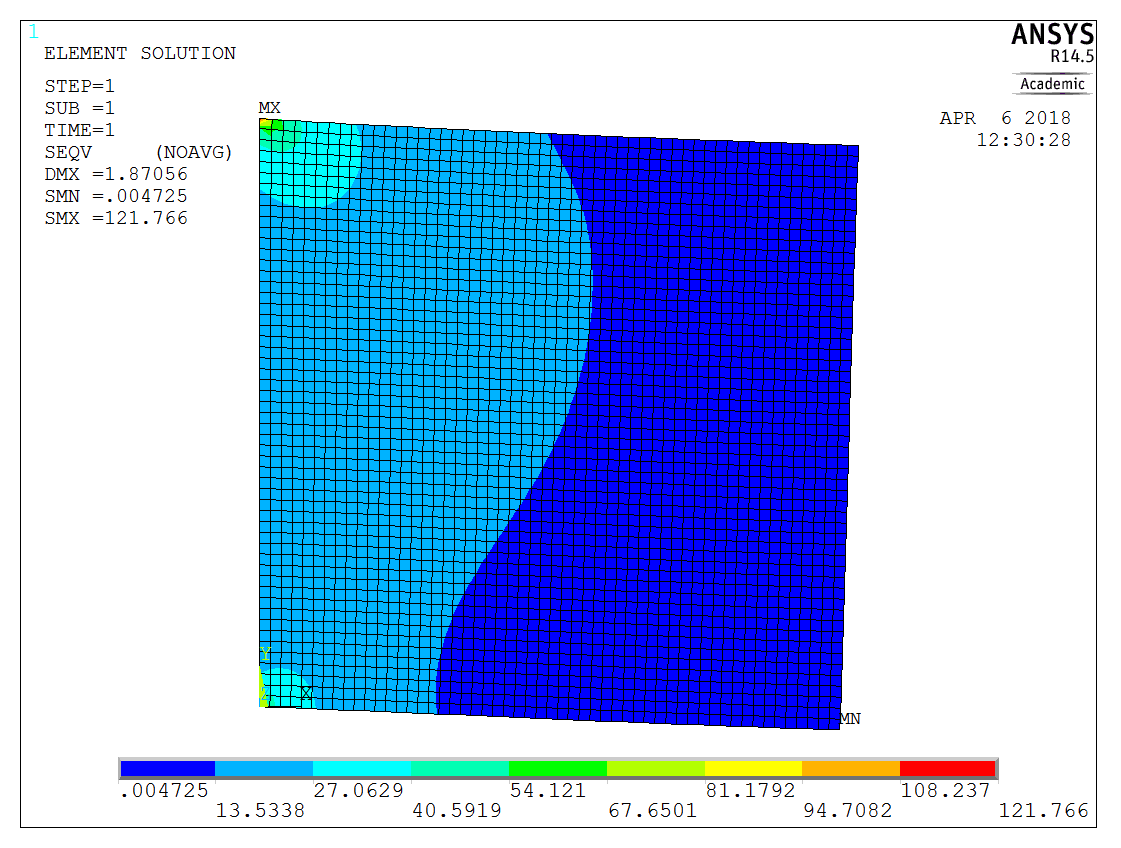
\includegraphics{adaptivity/ex_images/ex_short_cantilever_stress_ansys.png}
    }
    \caption{Von-mises stress contour using 9-node quadrilateral element in ANSYS (17930 DOFs)}
    \label{adap_fig:ex_chole_stress_ansys}
\end{figure}
\pagebreak